\section{Qualitative DDPM Samples}

\begin{figure}[H]
\centering
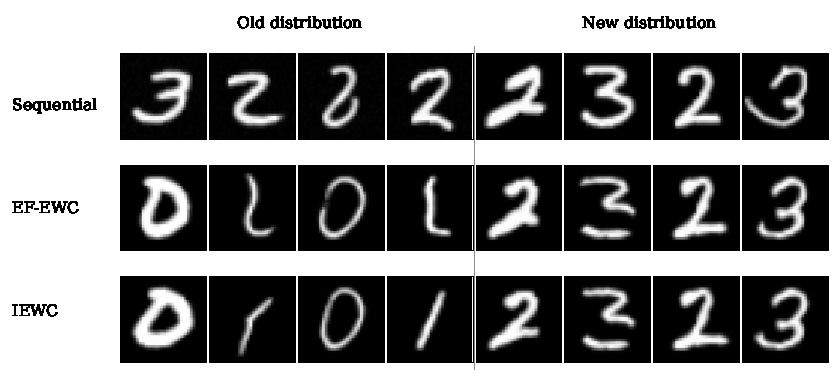
\includegraphics[width=0.66\linewidth]{figures/diffusion_generated_samples.pdf}
\caption[Diffusion generated samples]{Diffusion generated samples. The grid shows class-conditional MNIST generations from the DDPM architecture after a longer EMA training budget and continual training on both distributions. Rows compare sequential training, EF-EWC, and IEWC; columns show four old-distribution samples and four new-distribution samples. The old column alternates labels 0 and 1, and the new column alternates labels 2 and 3. Sequential training produces recognizable new-distribution digits but old-label samples drift toward new-distribution digits. EF-EWC and IEWC preserve old-label generations while learning recognizable new-label samples. This MNIST setting does not support the pattern reported in Rank1Diffusion, where EWC alone struggles in diffusion continual learning and diagonal EWC is ineffective relative to rank-1 Fisher regularization with generative distillation \protect\citep{Rank1Diffusion}.}
\label{fig:diffusion-generated-samples}
\end{figure}
